% Vector source for the primary-configuration speed--performance figure.
% Values are transcribed without recomputation from the locked seed-42
% performance and complexity tables in main.tex.
\documentclass[tikz,border=4pt]{standalone}
\usepackage{pgfplots}
\pgfplotsset{compat=1.18}
\usepgfplotslibrary{groupplots}
\definecolor{ezeroblue}{HTML}{4C78A8}
\definecolor{ethreered}{HTML}{E45756}
\definecolor{esixgreen}{HTML}{54A24B}

\begin{document}
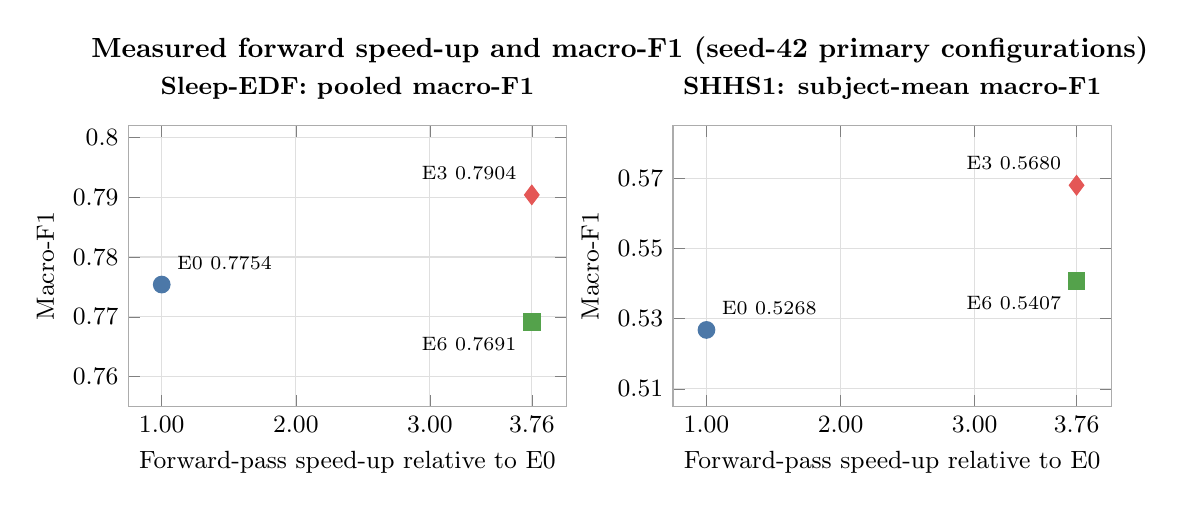
\begin{tikzpicture}
\begin{groupplot}[
  group style={group size=2 by 1,horizontal sep=1.35cm},
  width=7.15cm,
  height=5.15cm,
  xmin=0.75,xmax=4.02,
  xtick={1,2,3,3.76},
  xticklabels={1.00,2.00,3.00,3.76},
  xlabel={Forward-pass speed-up relative to E0},
  ylabel={Macro-F1},
  grid=both,
  minor grid style={gray!12},
  major grid style={gray!25},
  axis line style={gray!65},
  tick label style={font=\small},
  label style={font=\small},
  title style={font=\small\bfseries,align=center},
  clip=false
]

\nextgroupplot[
  title={Sleep-EDF: pooled macro-F1},
  ymin=0.755,ymax=0.802,
  ytick={0.76,0.77,0.78,0.79,0.80}
]
\addplot[only marks,mark=*,mark size=3pt,ezeroblue] coordinates {(1.00,0.7754)};
\node[font=\scriptsize,above right=2pt] at (axis cs:1.00,0.7754) {E0 0.7754};
\addplot[only marks,mark=diamond*,mark size=3.5pt,ethreered] coordinates {(3.76,0.7904)};
\node[font=\scriptsize,above left=2pt] at (axis cs:3.76,0.7904) {E3 0.7904};
\addplot[only marks,mark=square*,mark size=3pt,esixgreen] coordinates {(3.76,0.7691)};
\node[font=\scriptsize,below left=2pt] at (axis cs:3.76,0.7691) {E6 0.7691};

\nextgroupplot[
  title={SHHS1: subject-mean macro-F1},
  ymin=0.505,ymax=0.585,
  ytick={0.51,0.53,0.55,0.57}
]
\addplot[only marks,mark=*,mark size=3pt,ezeroblue] coordinates {(1.00,0.5268)};
\node[font=\scriptsize,above right=2pt] at (axis cs:1.00,0.5268) {E0 0.5268};
\addplot[only marks,mark=diamond*,mark size=3.5pt,ethreered] coordinates {(3.76,0.5680)};
\node[font=\scriptsize,above left=2pt] at (axis cs:3.76,0.5680) {E3 0.5680};
\addplot[only marks,mark=square*,mark size=3pt,esixgreen] coordinates {(3.76,0.5407)};
\node[font=\scriptsize,below left=2pt] at (axis cs:3.76,0.5407) {E6 0.5407};

\end{groupplot}
\node[font=\normalsize\bfseries] at ($(group c1r1.north)!0.5!(group c2r1.north)+(0,0.95cm)$)
  {Measured forward speed-up and macro-F1 (seed-42 primary configurations)};
\end{tikzpicture}
\end{document}
